\documentclass[10pt, landscape]{article}
\usepackage[scaled=0.92]{helvet}
\usepackage{calc}
\usepackage{multicol}
\usepackage{ifthen}
\usepackage[a4paper,margin=5mm,portrait]{geometry}
\usepackage{amsmath,amsthm,amsfonts,amssymb}
\usepackage{color,graphicx,overpic}
\usepackage{hyperref}
\usepackage{newtxtext} 
\usepackage{enumitem}
\usepackage[table]{xcolor}
\usepackage{mathtools}

\usepackage[outputdir=../]{minted} % for code syntax highlighting
\usepackage{mdframed} % framing, backgrounds

\setlist{nosep}

% for including images
\graphicspath{ {./images/} }


% \pdfinfo{
%   /Title (CS2040S.pdf)
%   /Creator (TeX)
%   /Producer (pdfTeX 1.40.0)
%   /Author (Zeepheru)
%   /Subject (CS2040S)
%   /Keywords (CS2040S, nus,cheatsheet,pdf)}

% Turn off header and footer
\pagestyle{empty}

\newenvironment{tightcenter}{%
  \setlength\topsep{0pt}
  \setlength\parskip{0pt}
  \begin{center}
}{%
  \end{center}
}

% redefine section commands to use less space
\makeatletter
\renewcommand{\section}{\@startsection{section}{1}{0mm}%
                                {-1ex plus -.5ex minus -.2ex}%
                                {0.5ex plus .2ex}%x
                                {\normalfont\large\bfseries}}
\renewcommand{\subsection}{\@startsection{subsection}{2}{0mm}%
                                {-1explus -.5ex minus -.2ex}%
                                {0.5ex plus .2ex}%
                                {\normalfont\normalsize\bfseries}}
\renewcommand{\subsubsection}{\@startsection{subsubsection}{3}{0mm}%
                                {-1ex plus -.5ex minus -.2ex}%
                                {1ex plus .2ex}%
                                {\normalfont\small\bfseries}}%
\renewcommand{\familydefault}{\sfdefault}
\renewcommand\rmdefault{\sfdefault}
%  makes nested numbering (e.g. 1.1.1, 1.1.2, etc)
\renewcommand{\labelenumii}{\theenumii}
\renewcommand{\theenumii}{\theenumi.\arabic{enumii}.}
\renewcommand\labelitemii{•}
\renewcommand\labelitemiii{•}
%  convenient absolute value symbol
\newcommand{\abs}[1]{\vert #1 \vert}
%  convenient floor and ceiling
\newcommand{\floor}[1]{\lfloor #1 \rfloor}
\newcommand{\ceil}[1]{\lceil #1 \rceil}
%  convenient modulo
\newcommand{\Mod}[1]{\ \mathrm{mod}\ #1}
%  for logical not operator, iff symbol, convenient "if/then"
\renewcommand{\lnot}{\mathord{\sim}}
\let\then\rightarrow
\let\Then\Rightarrow
%  vectors
\newcommand{\vv}[1]{\boldsymbol{#1}}
\newcommand{\VV}[1]{\overrightarrow{#1}}
%  column vector
\newcommand{\cvv}[1]{\left(\begin{smallmatrix}#1\end{smallmatrix}\right)}
\newcommand{\code}[1]{\textcolor{mygreen}{\texttt{#1}}}
\newcommand{\java}[1]{\mintinline{java}|#1|}
\newcommand\bggreen{\cellcolor{green!10}}

\makeatother
\definecolor{myblue}{cmyk}{1,.72,0,.38}
\definecolor{mygreen}{cmyk}{0.0, 0.66, 0.30, 0.33}
\everymath\expandafter{\the\everymath \color{myblue}}
% Define BibTeX command
\def\BibTeX{{\rm B\kern-.05em{\sc i\kern-.025em b}\kern-.08em
    T\kern-.1667em\lower.7ex\hbox{E}\kern-.125emX}}

% Don't print section numbers
\setcounter{secnumdepth}{0}

\setlength{\parindent}{0pt}
\setlength{\parskip}{0pt plus 0.5ex}
%% this changes all items (enumerate and itemize)
\setlength{\leftmargini}{0.5cm}
\setlength{\leftmarginii}{0.4cm}
\setlength{\leftmarginiii}{0.5cm}
\setlist[itemize,1]{leftmargin=2mm,labelindent=1mm,labelsep=1mm}
\setlist[itemize,2]{leftmargin=3mm,labelindent=1mm,labelsep=1mm}
\setlist[itemize,3]{leftmargin=3mm,labelindent=1mm,labelsep=1mm}

%My Environments
\newtheorem{example}[section]{Example}

% -----------------------------------------------------------------------

\begin{document}
\raggedright
\footnotesize
\begin{multicols}{2}

% multicol parameters
% These lengths are set only within the two main columns
\setlength{\columnseprule}{0.25pt} % column separator line
\setlength{\premulticols}{1pt}
\setlength{\postmulticols}{1pt}
\setlength{\multicolsep}{1pt}
\setlength{\columnsep}{2pt}

\begin{center}
    \fbox{%
        \parbox{0.8\linewidth}{\centering \textcolor{black}{
            {\Large\textbf{CS2030S}}
            \\ \normalsize{AY23/24S2 Final Examination}}
            \\ {\footnotesize By: \textcolor{myblue}{github.com/zeepheru}}
        }%
    }
\end{center}

% START CONTENT _________________________________>
\section{"Java"}
\begin{multicols}{2}

\textbf{Final}
\begin{itemize}
    \item Class - cannot be inherited.
    \item Method - cannot be overwritten.
    \item Field - cannot be reassigned.
\end{itemize}

\textbf{Static}
\begin{itemize}
    \item Fields - class fields.
    \item Methods: Accessed through class, cannot access non-static fields. 
\end{itemize}

\columnbreak{}

\textbf{Abstract}
\begin{itemize}
    \item Abstract class cannot be instantiated.
    \item Only \textbf{one} method needs to be abstract. 
    \item $\geq 1$ method is abstract \\ $\implies$ class HAS to be abstract!
\end{itemize}

\textbf{Interface}
\begin{itemize}
    \item All methods in an interface are \code{public abstract} by default.
    \item \java{I i2 = (I) new A()} would always compile - Compiler thinks \code{A} may implement \code{I}. 
\end{itemize} 
\end{multicols}

\vspace{3 pt}
\textbf{NOTE}: \java{private} fields/methods are \textbf{not} inherited by children classes. 
\vspace{3 pt}

\textbf{Primitives}
\begin{itemize}
    \item \code{byte <: short <: int <: long <: float <: double}
    \item \code{char <: int}
\end{itemize}



% a----------------------
\section{Signatures, Overriding/loading}
\textbf{Method Signature:}
\begin{itemize}
    \item \textbf{YES}: name, number of args, type of args, order of args
    \item \textbf{NO}: name of args, return type, exceptions
    \item Note: generics make a signature different.
    \item \textbf{Method Descriptor}: method signature \& return type.
\end{itemize}

\vspace{2 pt}
An \textbf{overridding} method:
\begin{itemize}
    \item NOT REQUIRED to throw the same exceptions.
    \item CANNOT be private if parent method is public.
    \item CAN return a subtype.
\end{itemize}
You cannot overload with the same arg types \textbf{after type erasure}. 
\begin{minted}{java}
    // Same signature after type erasure!
    void foo(A<String> a) {...} 
    void foo(A<Integer> a) {...}
\end{minted}


% a----------------------
\section{OOP Principles}
\textbf{Encapsulation, Composition, Inheritance\\}
\textbf{Polymorphism}
\begin{itemize}
    \item Method overriding - change how existing code behaves w/o changing the code itself
\end{itemize}
\textbf{Information Hiding}
\begin{itemize}
    \item \textit{“Abstraction barrier”, “publicly accessible”}
\end{itemize}
\textbf{Tell Don't Ask}
\begin{itemize}
    \item basically, never ask for the internals for a computation or operation
    \item Eg: an \code{Interval} and a \code{Time} → Don’t ask for the secs and ms from \code{Time} to compute differences, get \code{Time} \textbf{to do it itself}.
\end{itemize}
\textbf{Liskov Substitution Principle}
\begin{itemize}
    \item Let $\varphi(x)$ be a property provable about objects $x$ of type $T$. Then $\varphi(y)$ should be true for objects $y$ of type $S$ where $S<:T$.
    \item $A$ subclass should not break the expectations set by the superclass. If a class $B$ is substitutable for a parent class $A$, then it should be able to pass all test cases of the parent class $A$. If it does not, it is not substitutable → LSP is violated.
    \item Any code written for $A$ would still work if we substitute $A$ with $B$.
\end{itemize}

% --------------------------
\section{Misc-1}
\subsection{Dynamic Binding}
\begin{enumerate}
    \item At compile-time, find matching object descriptor in CTT.
    \item At run-time, find a method with the same method descriptor in RTT.
\end{enumerate}

\subsection{Varargs}
\begin{itemize}
    \item \java{void foo(T... args)} - \code{args} will be \code{T[]}.
    \item Use \java{@SafeVarargs} for when \code{T} is generic. 
\end{itemize}

\subsection{Variances}
\begin{itemize}
    \item \textbf{Covariant}: $ S <: T \implies C(S) <: C(T)$
    \begin{itemize}
        \item E.g. \code{arrays}
    \end{itemize}
    \item \textbf{Contravariant}: $ S <: T \implies C(T) <: C(S)$
    \item \textbf{Invariant}: Neither.
    \begin{itemize}
        \item E.g.\code{generic classes}
    \end{itemize}
\end{itemize}

% a----------------------
\section{Generics, Wildcards}
Wildcards can be in return types. \\ 
Generics are generally invariant.

\subsection{Upper-bounded Wildcard}
\begin{itemize}
    \item\textbf{\java{Seq<? extends Shape>}}.
    \item For any type \code{S}, \code{A<S>} $<:$ \code{A<? extends S>}
    \item Covariance: if \code{S} $<:$ \code{T}, then \code{A<? extends S>} $<:$ \code{A<? extends T>}.
    \item So in practice, an argument \code{Seq<? extends T>} would match \code{Seq<T>} and \code{Seq<S>}, where \code{S} $<:$ \code{T}.
\end{itemize}
\subsection{Lower-bounded Wildcard}
\begin{itemize}
    \item \textbf{\java{Seq<? super Shape>}}
    \item For any type \code{S}, \code{A<S>} $<:$ \code{A<? super S>}
    \item Contravariance: if \code{S} $<:$ \code{T}, then \code{A<? super T>} $<:$ \code{A<? super S>}.
\end{itemize}



\subsection{PECS}
Producer \code{extends}; Consumer \code{super}.

\subsection{Type Erasure}
\begin{minted}{java}
    Integer i = A<String>.foo();
    // becomes
    Integer i = (Integer) A.foo();
\end{minted}
Hence why you can't do \java{a instanceof A<String>}.
\\
\vspace{2 pt}
\textbf{Generics and Arrays \\}
arrays are reifiable - full type information should be available at runtime - now type erasure complicates matters - the generic is gone.
\\ \java{new A<?>[10]} works because it is reifiable!

\section{Exceptions}
\textbf{Potential Issues}
\begin{enumerate}
    \item Using exceptions as \textit{control flow}.
    \item Catching \textbf{all} possible exceptions - not advisable.
    \item Anticipated exceptions should be a \textbf{checked exception}.
\end{enumerate}

\section{Nesting}
\begin{itemize}
    \item \textbf{Inner} class: non-static class in \code{class}. 
    \begin{itemize}
        \item Consider a $B$ in an $A$.
        \item \code{A.B b = a. new B()} is valid initialization code, where \code{A a = new A();}
        \item \code{this} in \code{B} would refer to \code{B}.
        \item To access the fields of \code{A} use the \textit{qualified reference} \code{A.this}.
        \item Not using a \textit{qualified reference} is fine.
        \item The \textbf{same name} can be used inside and outside an inner class - the closest innermost one will be used. 
    \end{itemize}
    \vspace{2 pt}
    \item \textbf{STATIC nested} class - Operates similarly to a static method. Can only access static fields and methods in outer class. 

    \vspace{2 pt}
    \item \textbf{Local} class: class in \code{method}. 
    \begin{itemize}
        \item Variable capture:
        \begin{itemize}
            \item Captures the fields from outer method \textbf{that it needs}. 
            \item Field has to be \textbf{final} or \textbf{implicitly final} - no reassignment after first initialisation.
            \item Always captures the outer class of the method: \java{B.this}
        \end{itemize}
    \end{itemize}
    
\end{itemize}

\subsection{Anonymous Class}
\begin{multicols}{2}
Extending class:
\begin{minted}{java}
new Book("name") {
    @Override
    public String foo() {
        ...
    }
}
\end{minted}
\columnbreak

Implementing interface:
\begin{minted}{java}
new Runnable() {
    @Override
    public void run() {
        ...
    }
}
\end{minted}
\end{multicols}

% ......................
\section{Monads}
\code{map} - $X \to Y$ $\|$ \code{flatMap} - $X \to Monad(Y)$ \\
\vspace{3 pt}

\textbf{Left Identity Law}
\begin{itemize}
    \item $id \circ f=f$
    \item \java{Monad.of(x).flatMap(y -> G(y)) = G(Y)}
\end{itemize}
\textbf{Right Identity Law}
\begin{itemize}
    \item $f \circ id = f$
    \item \java{m.flatMap(x -> Monad.of(x)) = m}
\end{itemize}
\textbf{Associative Law}
\begin{itemize}
    \item \java{m.flatMap(x -> F(x)).flatMap(y -> G(y))} 
    \item \java{ = m.flatMap(x -> F(x).flatMap(y -> G(y)))}
\end{itemize}
\vspace{3 pt}
\textbf{Preventing violating of laws}
\begin{itemize}
    \item The \code{flatMap} method should \textbf{NOT add anything on its own} - would violate associative law
    \begin{itemize}
        \item \textit{eg add some string to the log}
        \item \textbf{It should just combine/operate on previous values/side info}
    \end{itemize}
    \item The \code{of} method should \textbf{NOT add anything either}
    \begin{itemize}
        \item \textit{eg its own startup message}
    \end{itemize}
\end{itemize}


\subsection{Functors}
Lambdas can be applied sequentially to a value; does not carry side info. 
\begin{itemize}
    \item Supports a \code{map} and \code{of}.
    \item \textbf{Preserving Identity}: \code{functor.map(x -> x)} is the same as \code{functor}
    \item \textbf{Preserving Composition}: \code{functor.map(x -> f(x)).map(x -> g(x))} is the same as \code{functor.map(x -> g(f(x))}.
\end{itemize}
\textbf{Rec. Note}: Monads are functors. You can write \code{map} using \code{flatMap}!


% a----------------------
\section{Lambdas}
\java{ff -> x -> ff.transform(x); } is correct syntax. \\ 
In fact, this, $f:X \to Y \to Z$, returning a sequence of $n$ unary functions, is called \textbf{"currying"}.
\subsection{Funtional Interface}
\begin{itemize}
    \item \code{@FunctionalInterface}
    \item Exactly 1 \textbf{abstract} method. (can contain other stuff)
\end{itemize}

% ______________________
\section{Immutability}
\begin{itemize}
    \item Fields \code{final}; always \code{return} \textbf{new instance} of obj. 
    \begin{itemize}
        \item \textbf{Ease of understanding} - guarantees obj being passed around is the same.
        \item \textbf{Safe sharing of objects} - eg an origin is always the same.
        \item \textbf{Safe sharing of internals}
        \item \textbf{Safe concurrent exec}
    \end{itemize}
\end{itemize}

% a----------------------
\section{Parallel/Async}
\begin{itemize}
    \item \textbf{Concurrency} - divides computation into subtasks called threads.
    \item \textbf{Parallelism} - multiple subtasks/threads running at the same time.
    \item parallelism $\subseteq$ concurrency
\end{itemize}

\subsection{Threads}
New \java{Thread().start()}'s are async.
\begin{minted}{java}
    // A and B in any order
    new Thread(() -> printRepeat("A")).start();
    new Thread(() -> printRepeat("B")).start();
    // Also
    System.out.println(Thread.currentThread().getName()); 
\end{minted}


\subsection{CompletableFuture}
Chaining \java{cF.thenApplyAsync().thenApplyAsync()...} will be done \textbf{in order}!
\\ Also note the necessity to \java{join()} at the end. Otherwise not all will be printed. 

\subsection{ForkJoin}
Always preferable to \code{fork} then \code{join} in a different order. Highest level of parallelism.
\begin{minted}{java}
    right.fork(); left.fork();
    return mid.compute() + right.join() + left.join();
\end{minted}

\textbf{ForkJoinPool}

\begin{itemize}
    \item Each thread has a deque of tasks.
    \item When a thread is idle, it checks its deque of tasks. If the deque is not empty, it picks up a task at the head of the deque to execute \textit{(e.g., invoke its \code{compute()} method).}
    \item Otherwise, if the deque is empty, it picks up a task from the \textit{tail} of the deque of another thread to run. The latter is a mechanism called \textbf{work stealing}.
    \item When \code{fork()} is called, the caller adds itself to the \textit{head} of the deque of the executing thread. This is done so that the most recently forked task gets executed next, similar to how normal recursive calls.
    \item When \code{join()} is called, several cases might happen. If the subtask to be joined hasn't been executed, its \code{compute()} method is called and the subtask is executed.
    \begin{itemize}
        \item If the subtask to be joined has been completed (some other thread has stolen this and completed it), then the result is read, and \code{join()} returns.
        \item If the subtask to be joined has been stolen and is being executed by another thread, then the current thread either finds some other tasks to work on from its local deque, or steals another task from another deque.
    \end{itemize}
\end{itemize}




\end{multicols}

\hline
\section{Stack and Heap Examples}
\begin{multicols}{4}
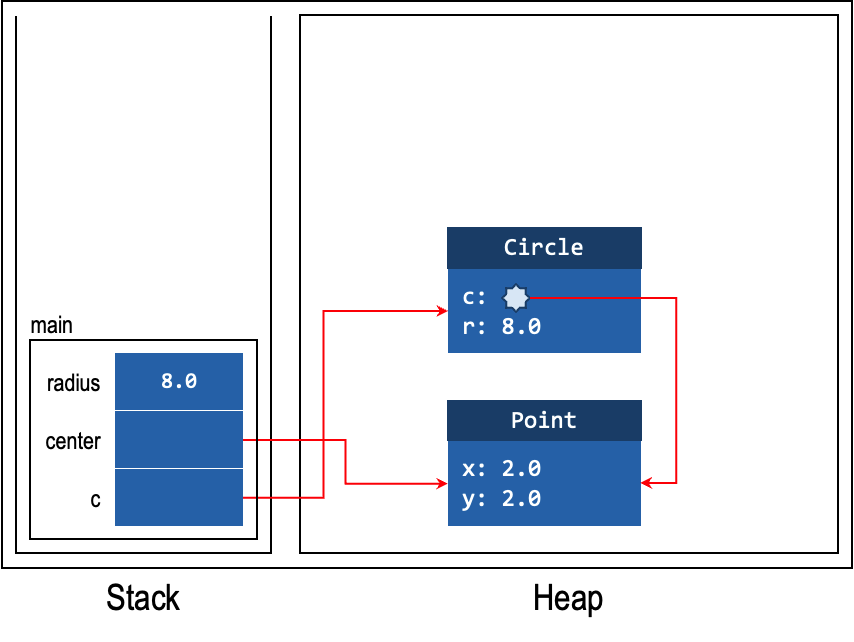
\includegraphics[scale=0.15]{sh1}
\columnbreak
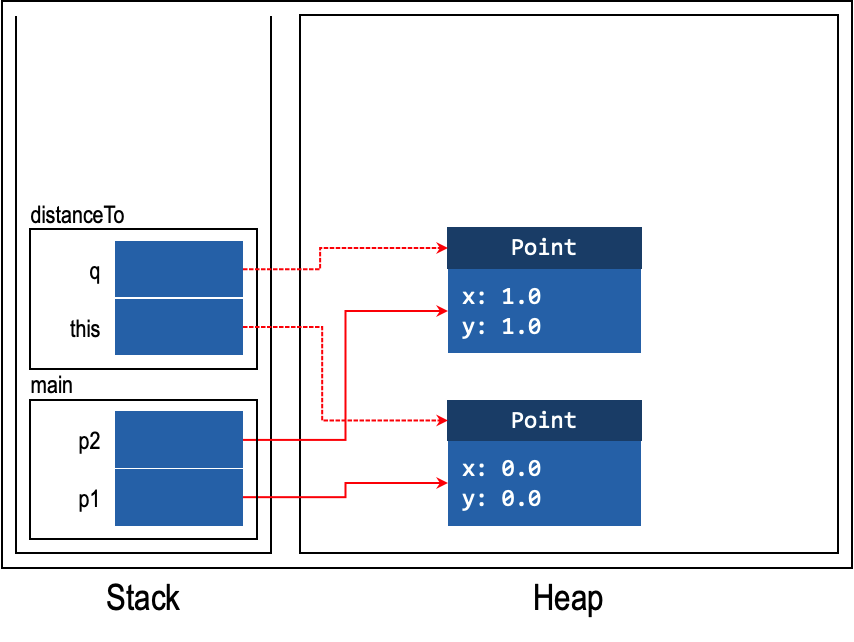
\includegraphics[scale=0.15]{sh2}
\columnbreak
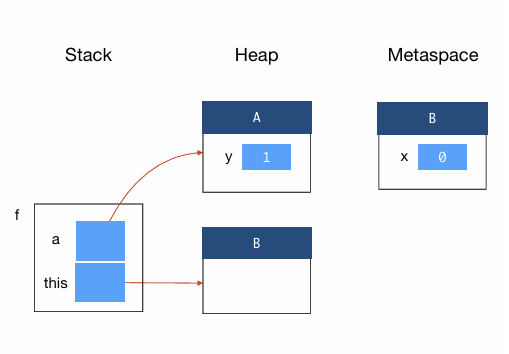
\includegraphics[scale=0.35]{sh3}
\columnbreak
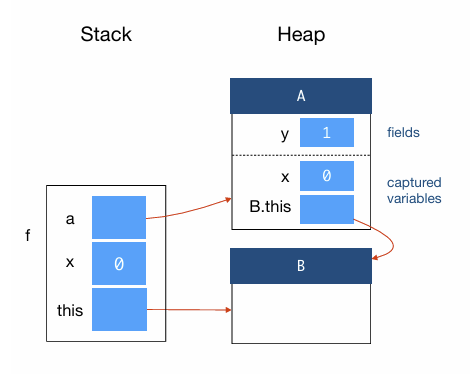
\includegraphics[scale=0.35]{sh4}
\end{multicols}

\end{document}

